\documentclass[a4paper]{article}
\usepackage{amsthm}
\usepackage{amsmath} % Define various maths environments
\usepackage{amssymb} % Define various maths symbols
\usepackage{mathrsfs}
\usepackage{geometry} % Adjust the margin, paper size, and etc.
\usepackage{enumerate} % Provide different style of lists
\usepackage{graphicx}
\usepackage{float}
\usepackage{multirow}
\geometry{a4paper,scale=0.78}

\title{—————————————————————————\\ \sc{UM-SJTU Joint Institute}}
\author{\sc{Computer Networks}}
\date{\sc{(Ve489)}\\——————————————————————————————}

\begin{document}
\maketitle
\vspace{5cm}
\centerline{\Large{\sc{Mini-Project 2 Report}}}
\vspace{9cm}
\begin{tabular}{lll}
\qquad \qquad Name: Sun Yiwen&ID: 517370910213\\
\qquad \qquad Date: Aug 4 2020
\end{tabular}

\newpage
\section{Step 3: TCP Segment Structure}
\begin{figure}[htbp]
\centering
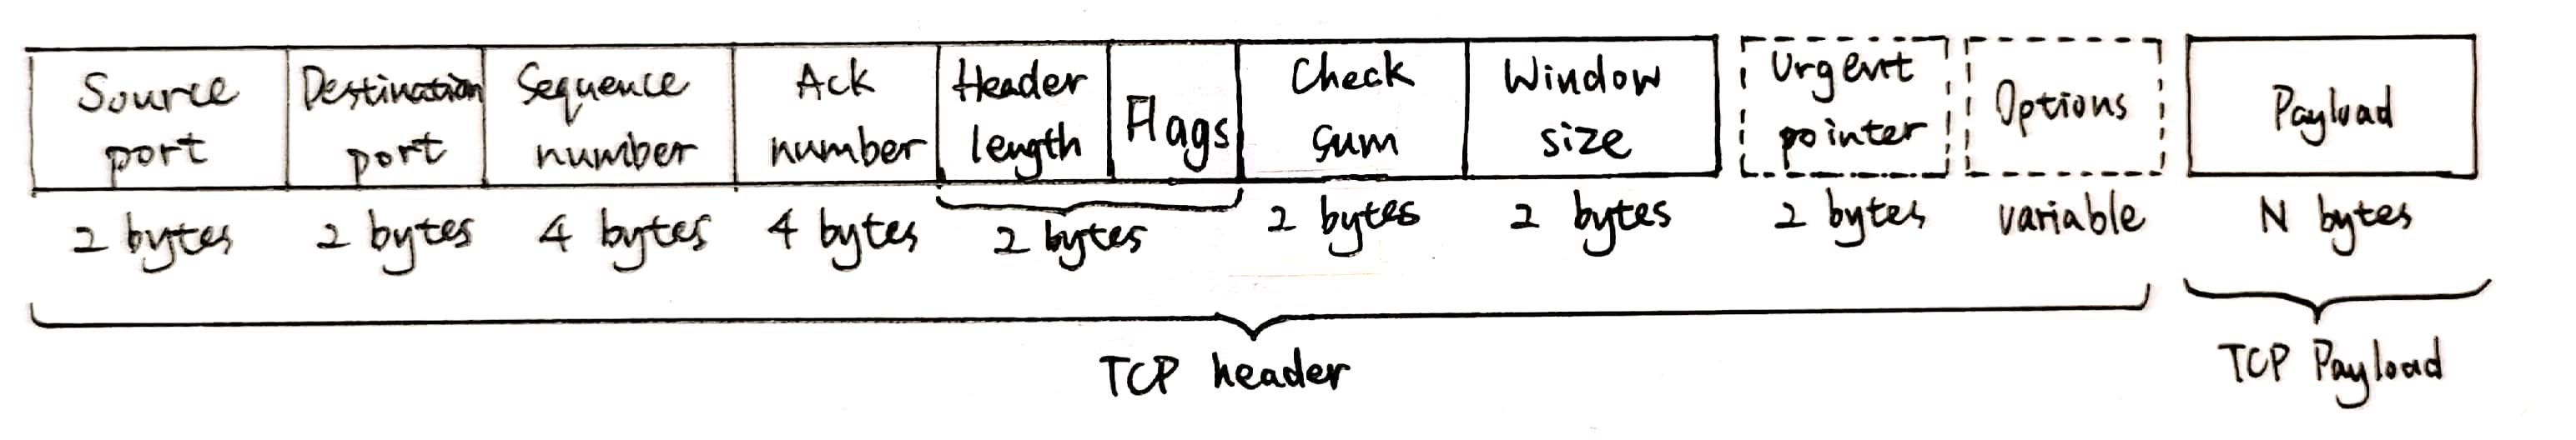
\includegraphics[scale=0.15]{1.jpg}
\caption{My drawing of a TCP segment.}
\end{figure}
\section{Step 4: TCP Connection Setup/Teardown}
\begin{figure}[htbp]
\centering
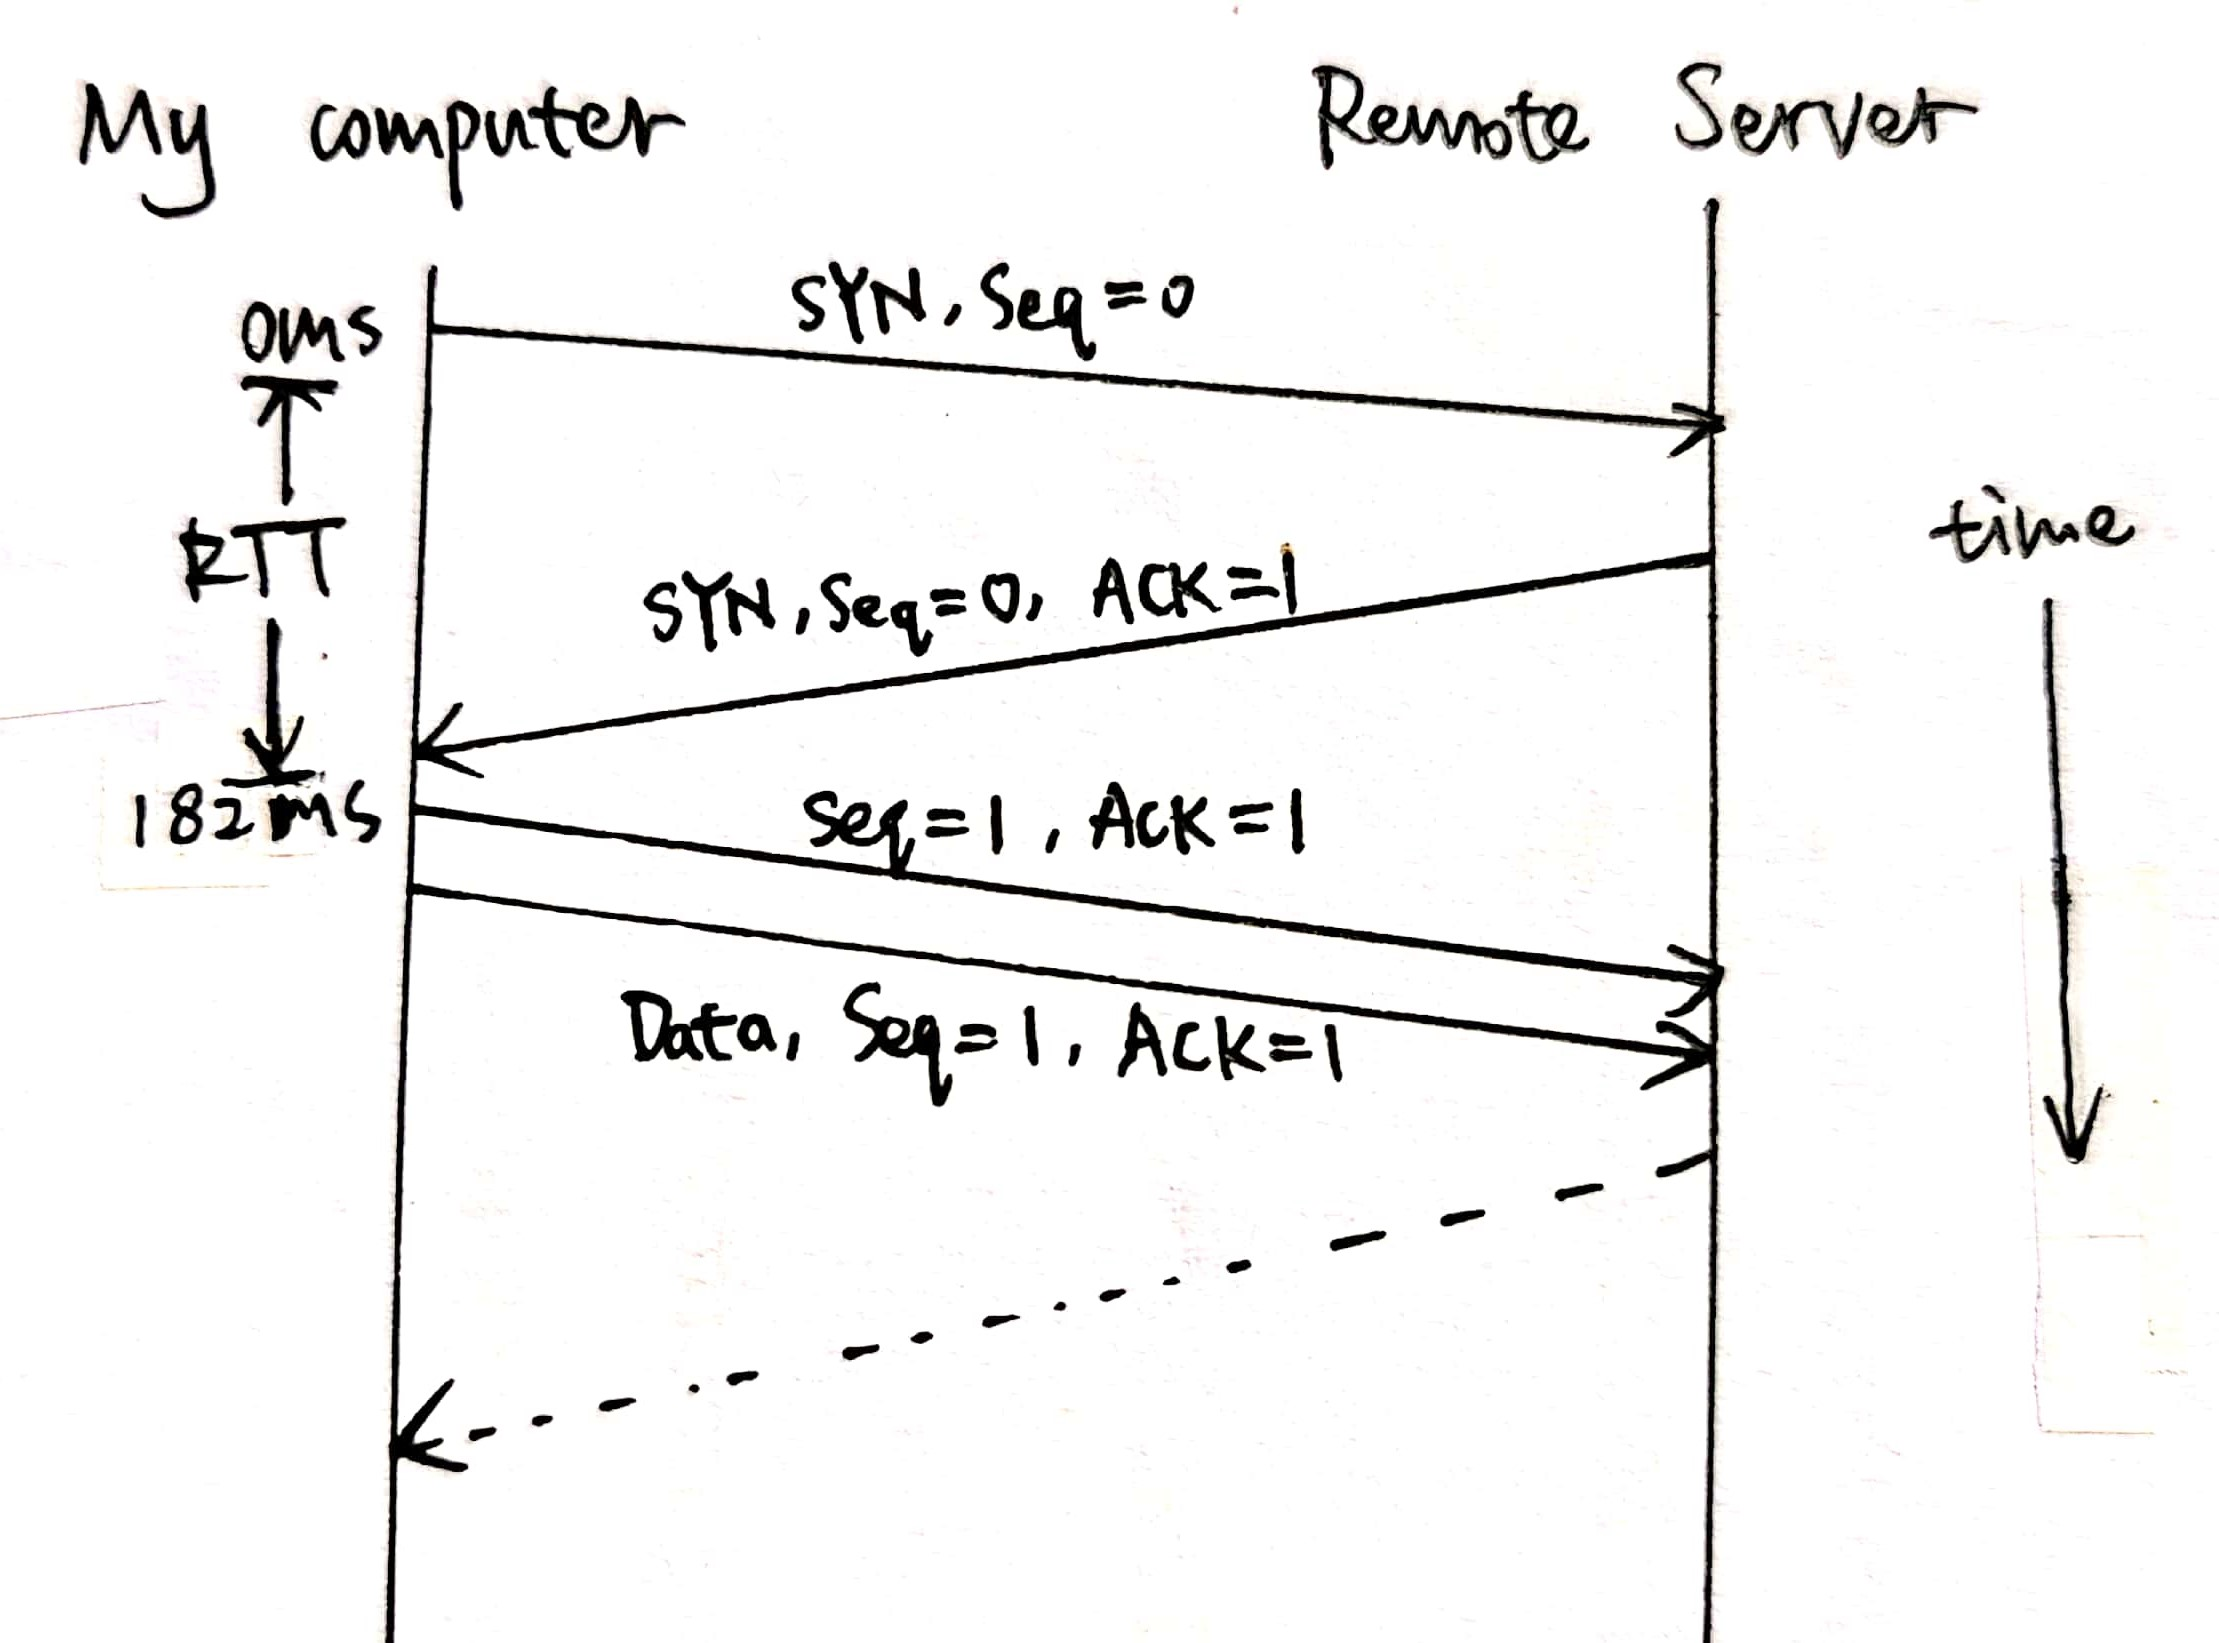
\includegraphics[scale=0.1]{2.jpg}
\caption{My drawing of a time sequence diagram of the three-way handshake.}
\end{figure}
\subsection{Connection Options}
The TCP Options are Maximum segment size, SACK permitted, Timestamps, and Window scale. They are used in both directions.
\subsection{FIN/RST Teardown}
\begin{figure}[htbp]
\centering
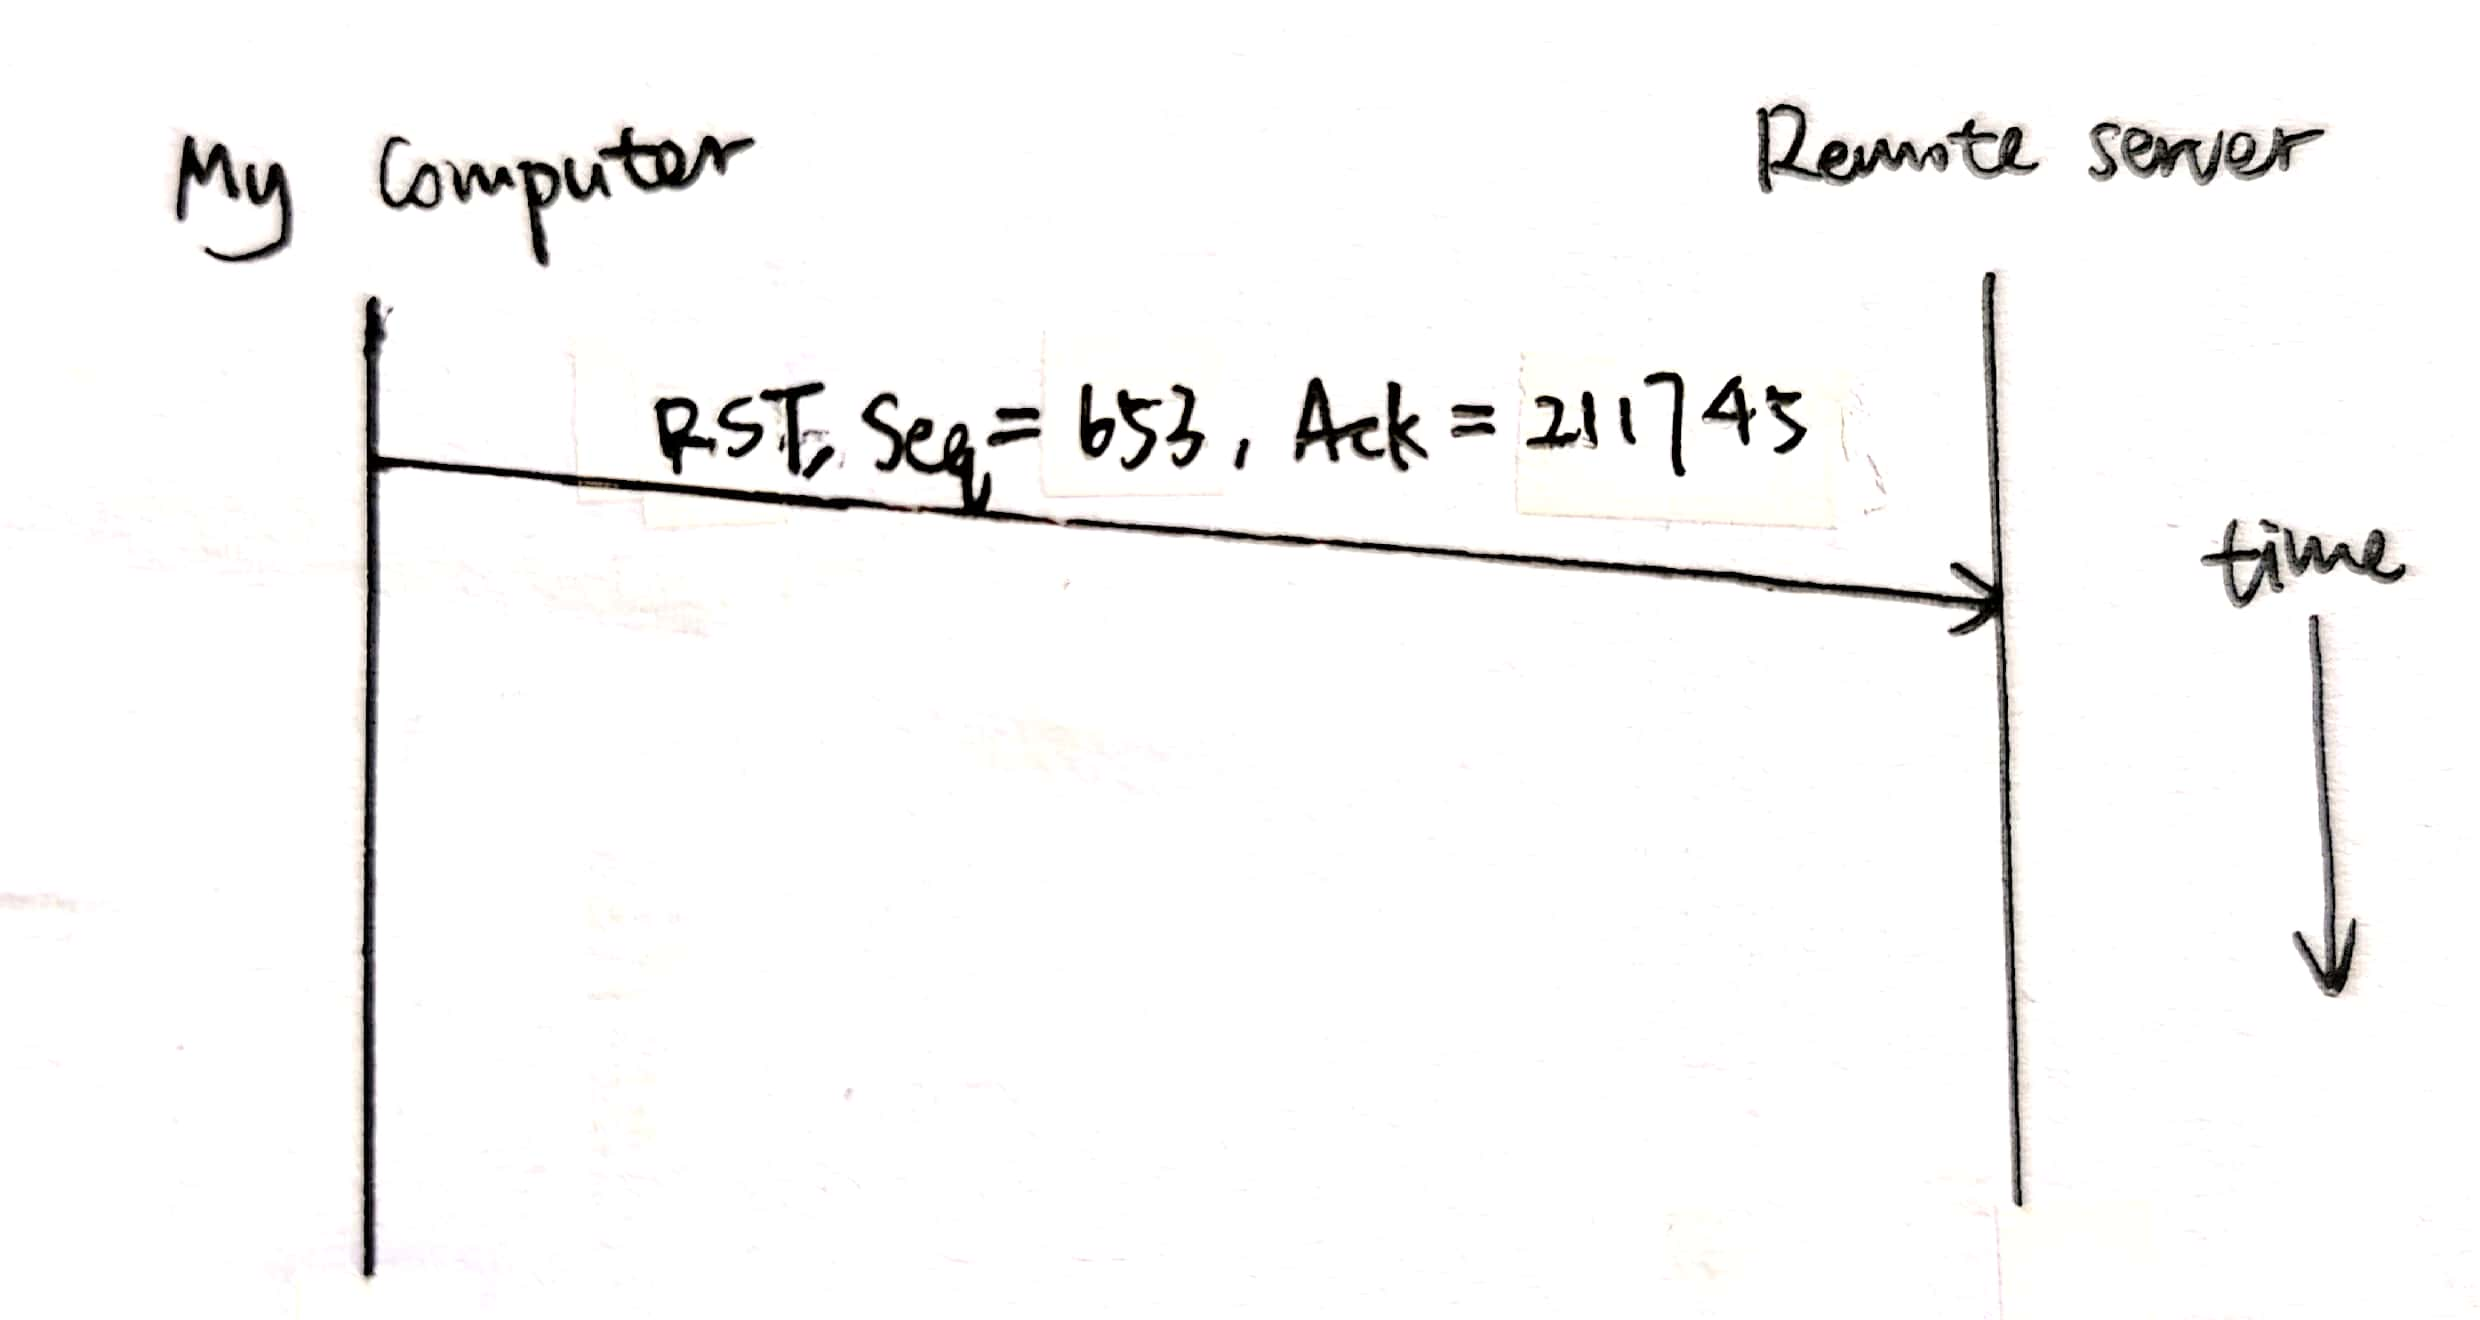
\includegraphics[scale=0.09]{3.jpg}
\caption{My drawing of the teardown.}
\end{figure}
\section{Step 5: TCP Data Transfer}
\begin{enumerate}
\item
The data rate in the download direction is 37 packets/second and 370Kbps.
\item
A typical download packet is 1494 bytes long and 1400 bytes are the TCP payload. Therfore, about 93$\%$ of this download rate is content.
\item
The data rate in the upload direction is 18 packets/second and 8500 bits/second.
\item
The ACK number that the next transmitted TCP segment carries will be $X+1400$, where 1400 is the TCP payload bytes.
\end{enumerate}


\end{document}